\section{Study 2: long-horizon degradation under calibrated difficulty}
\label{sec:study2}

Study~1 tasks span at most nine turns, and their difficulty is not controlled.
In long dialogues the questions themselves may become harder, so a falling
accuracy curve could reflect the questions rather than the context. Study~2
therefore uses a purpose-built benchmark with an exact answer at every turn and
difficulty set by design.

\subsection{The CDR-Stream benchmark and design}

\paragraph{Dialogues}
CDR-Stream contains 100-turn dialogues in four state-tracking domains: a budget
ledger, inventory across warehouses, a laboratory protocol with container
volumes, and chains of project milestones. Each user turn states events that
update a shared state, such as a delivery, a transfer or a correction, possibly
with distractor sentences, and asks one question: a sum, a difference, a count
above a threshold, a maximum, a what-if or a share. An exact solver computes
the gold answer of every turn.

\paragraph{Calibrated difficulty and scenarios}
Difficulty follows a 12-level ladder that changes one axis per step: query
terms, events per turn, distractors or event complexity (supplementary
Table~S4). Before any stream existed, a single-turn calibration
mapped easy, medium and hard regimes to ladder levels for each model and domain,
targeting accuracy bands of 0.75--0.92, 0.60--0.78 and 0.35--0.65, and a frozen
rule (isotonic fit, \citealp{barlow1972statistical}; one-sided Cochran--Armitage
trend test, \citealp{armitage1955tests}; minimum regime gaps) excluded domains
with a ceiling, a floor or no trend (supplementary Table~S5). Each
model is thus evaluated in its own informative range, at the cost of models not
all being tested on the same set of domains; CDR-Stream is not designed to
rank models against each other, and we do not compare raw accuracy across
models for this reason. Five scenarios fix the
regime sequence: stationary easy (S0-E) and hard (S0-H), which serve as
monitoring nulls; a staircase from easy to hard with changes at turns 34 and 68
(S1); a sudden easy-to-hard shift at turn 51 (S2); and easy to hard to easy
with changes at 34 and 67 (S3); within a regime, levels are mixed around the
centre level (supplementary Section~S2.2).

\paragraph{Models, arms and analysis}
GPT-4o-mini, Llama-3 70B \citep{grattafiori2024llama3} and Gemma 3 12B
\citep{gemma2025gemma3} were retained because they passed calibration and a
technical pilot, before any stream outcome existed; replaced candidates and two
disclosed deviations for Llama-3 70B are documented in the supplement. Each
model received 30 held-out dialogues, six per scenario, in two arms: dialogue
history, and the verified state summary with the current turn. Both arms used
the same prompt and contract (at most eight numbered reasoning lines followed by
\texttt{FINAL\_ANSWER: <integer>}), temperature 0.7 and a 2,048-token ceiling.
The dialogue arm also drew $K=3$ samples and $L=2$ rewordings per turn;
because the research budget staged acquisition, these were completed only for
GPT-4o-mini. Truncated replies were kept and scored as missing under a policy
frozen before the main run. Dialogues are the independent units. A
prespecified secondary contrast compares accuracy at turns 1--50 and 51--100 at
the same ladder level within each dialogue -- holding question-side difficulty
fixed (query terms, events per turn, distractors and event complexity), not
the conversation length or the accumulated state, since those grow across
turns under both arms by design. The confirmatory hypothesis H-C1 states that,
for Llama-3 70B and Gemma 3 12B, per-dialogue accuracy over turns 1--100 is
higher under the verified state summary, tested by one-sided sign-flip tests
over 30 dialogues (20,000 draws;
\citealp{good2005permutation}) with bootstrap intervals and Holm correction.
GPT-4o-mini control data had been seen before this protocol and are reported
outside the family.

\subsection{Results}

\paragraph{Accuracy collapses under accumulated history}
In all three models, dialogue-history accuracy fell from about 0.6 in the first
five turns to about 0.1 after turn 20 (Table~\ref{tab:s2collapse},
Figure~\ref{fig:s2}a). The curves of the three models were nearly identical
despite different sizes and mappings, and the collapse appeared in every
scenario. In stationary easy dialogues, where the questions never became
harder, accuracy over turns 21--100 was \cdrSzeroEDialRange{} under dialogue
history against \cdrSzeroECtrlRange{} under the verified state summary. At the
same ladder level, late turns were less accurate than early turns by
\cdrLevelMatched{} (prespecified secondary, $p$~\cdrLevelMatchedP{},
$n=\cdrLevelMatchedN$ dialogues; \cdrLevelMatchedSzeroE{} in S0-E). Because most
of the decline occurs in the first half, this contrast understates the total
loss. The collapse also hides the scheduled task drifts: it is present in
stationary dialogues and begins before any detector could form a baseline, so
pre/post contrasts around the scheduled changes mix the two (supplementary
Table~S7).

\begin{table}[!htbp]
\centering
\caption{Study 2 accuracy (CQ) by turn range under dialogue history, pooled and
in the stationary easy scenario (S0-E), and under the verified state summary
(turns 21--100). Thirty dialogues per model.}
\label{tab:s2collapse}
\small
\begin{tabular}{lccccc}
\toprule
 & \multicolumn{3}{c}{Dialogue history, turns} & S0-E, & State summary,\\
\cmidrule(lr){2-4}
Model & 1--5 & 6--20 & 21--100 & turns 21--100 & turns 21--100\\
\midrule
\inputtable{generated/table_cdr_collapse.tex}
\bottomrule
\end{tabular}
\end{table}

\begin{figure}[!htbp]
\centering
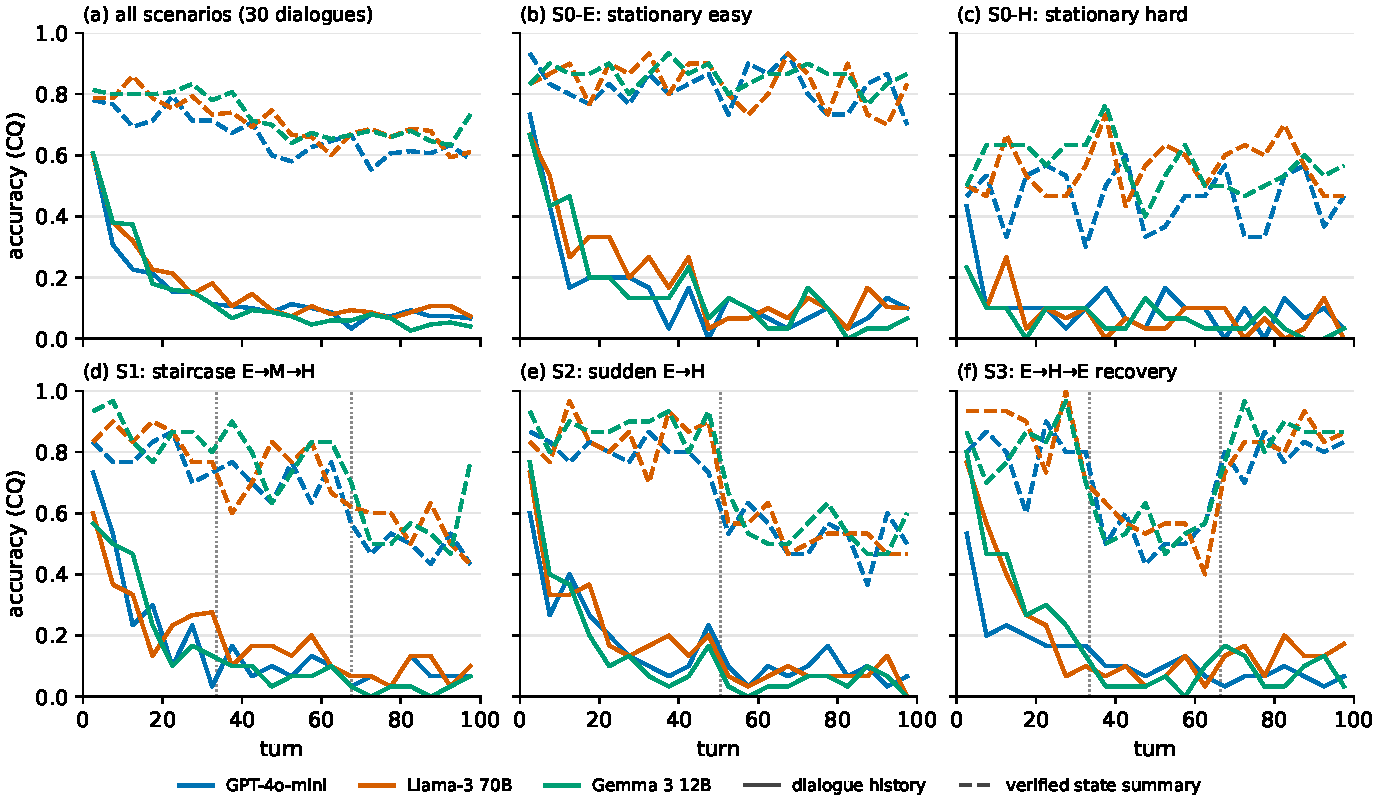
\includegraphics[width=\linewidth]{study2_accuracy_over_turns.pdf}
\caption{Study 2 accuracy over 100 turns in 5-turn bins: (a) all 30 dialogues
per model; (b)--(f) the five scenarios, six dialogues per model each. Solid:
dialogue history; dashed: verified state summary; dotted vertical lines:
scheduled difficulty changes.}
\label{fig:s2}
\end{figure}

\paragraph{A verified state summary preserves accuracy (confirmatory)}
Under the verified state summary, accuracy stayed high and followed the
difficulty schedule, stepping down at the changes of S1 and S2 and recovering in
the final easy regime of S3, a recovery that dialogue history never showed
(Figure~\ref{fig:s2}). H-C1 was supported for both members of the family
(Table~\ref{tab:s2control}): over turns 1--100 the gap was
\cdrLlamaControlGap{} for Llama-3 70B and \cdrGemmaControlGap{} for Gemma 3 12B
(Holm $p$~\cdrLlamaControlHolmP{} and \cdrGemmaControlHolmP{}), and over turns
21--100 it was \cdrLlamaControlLateGap{} and \cdrGemmaControlLateGap{}.
GPT-4o-mini showed the same direction.

\begin{table}[!htbp]
\centering
\caption{Frozen test H-C1: per-dialogue accuracy of the verified state summary
minus dialogue history over turns 1--100. GPT-4o-mini was observed before the
protocol and is outside the Holm family.}
\label{tab:s2control}
\small
\begin{tabular}{lcccc}
\toprule
Model & Mean gap & 95\% bootstrap CI & Holm $p$ & Dialogues\\
\midrule
\inputtable{generated/table_cdr_control_completion.tex}
\bottomrule
\end{tabular}
\end{table}
